\newcommand{\defs}{../defs}
\documentclass[12pt,oneside,chapterprefix=true]{scrbook}

\usepackage[T1]{fontenc}
\usepackage[utf8x]{inputenc}
\usepackage[brazilian]{babel}
\usepackage[table]{xcolor}
\usepackage{minted}
\usepackage[a5paper,left=0.7cm,right=0.7cm,top=2cm,bottom=2.5cm,]{geometry}
\usepackage{url}
\usepackage{graphicx}
\usepackage[export]{adjustbox}
\usepackage{hyperref}
\usepackage[square]{natbib}
\usepackage[parfill]{parskip}
\usepackage{mdframed}
\usepackage{longtable}
\usepackage{soul}
\usepackage{tabularx}
\usepackage[shortlabels]{enumitem}
\usepackage{xifthen}
\usepackage{multirow}
\usepackage[portuguese, ruled, vlined, linesnumbered, algochapter]{algorithm2e}
\usepackage{amsmath}
\usepackage{amssymb}
\usepackage{amsthm}
\usepackage{tablefootnote}
\usepackage{subfigure}
\usepackage{gensymb}
\usepackage{pgfplots}
\usepackage{xpatch}
\usepackage{varwidth}
\usepackage[htt]{hyphenat}

\renewcommand{\familydefault}{\sfdefault}

\newcommand{\name}{Prof. Marcelo de Souza}
\newcommand{\email}{marcelo.desouza@udesc.br}
\newcommand{\course}{Bacharelado em Engenharia de Software}
\newcommand{\university}{Universidade do Estado de Santa Catarina}
\newcommand{\campus}{Centro de Educação Superior do Alto Vale do Itajaí}
\newcommand{\shortuniversity}{UDESC Ibirama}
\newcommand{\version}{Versão compilada em \today}
\newcommand{\exercisedescription}{Exercício}

\usepackage[automark,headsepline,footsepline]{scrlayer-scrpage}
\lehead{\content}
\lohead{\content}
\rehead{}
\rohead{}
\cehead{}
\cohead{}
\lefoot{\name}
\lofoot{\name}
\refoot{\\\thepage}
\rofoot{\\\thepage}
\cofoot{}
\cefoot{}
\setkomafont{pagehead}{\normalfont\small}
\setkomafont{pagefoot}{\normalfont}

\newpairofpagestyles{firstpage}{}

\newcommand{\makeheader}{
	\thispagestyle{firstpage}
	\vspace*{-42pt}
	\framebox[\textwidth]{
		\parbox{0.97\textwidth}{
			\begin{center}
				{\scriptsize\shortcourse\ -- \class}
				
				\vspace{10pt}
				
				\textbf{\content}
				
				\vspace{2pt}
				
				{\small\name}
				
				\vspace{10pt}
				
				{\scriptsize\shortuniversity\hfill\email}
				
				\vspace{-5pt}
				
				{\scriptsize\course\hfill\version}
				
			\end{center}
		}
	}
%	\vspace{-15pt}
%	\begin{flushright}
%		{\scriptsize\source}
%	\end{flushright}
	\smallskip
}

\renewcommand{\thesection}{\arabic{section}}

\allowdisplaybreaks

\hypersetup{
	colorlinks,
	linkcolor={blue!80!black},
	citecolor={blue!80!black},
	urlcolor={blue!80!black}
}

\definecolor{codelinecolor}{gray}{.90}
\colorlet{codeboxcolor}{blue!8}

\surroundwithmdframed{minted}

\BeforeBeginEnvironment{mdframed}{}
\AfterEndEnvironment{mdframed}{}

\mdfsetup{%
	backgroundcolor=codeboxcolor,
	linecolor=white}

\setminted{%
	mathescape,
	escapeinside=@@,
	linenos,
	breaklines,
	tabsize=3,
	fontsize=\footnotesize}

\newcommand{\code}[1]{%
	\sethlcolor{codelinecolor}
	\texttt{\hl{#1}}%
}

\newcommand{\inblock}[1]{%
	\sethlcolor{blockcolor}
	\hl{\mbox{#1}}%
}

\newcommand{\javacode}[1]{%
	\mintinline[escapeinside=~~]{java}{#1}
}

\newcommand{\javacodecolor}[1]{%
	\mintinline[escapeinside=~~,bgcolor=codeboxcolor]{java}{#1}
}

\newcounter{number}
\newenvironment{exercise}[1][]
{%
	\refstepcounter{number}%
	\noindent%
	\ifthenelse{\equal{#1}{}}%
		{\textbf{\exercisedescription~\thenumber.\\}}%
		{\textbf{\exercisedescription~\thenumber. (#1)\\}}%
	\rmfamily%
}{\medskip}%

\newcommand{\resetexercisenumbering}{
	\setcounter{number}{0}
}

\newcounter{solutionnumber}
\newenvironment{solution}[1][]
{%
	\refstepcounter{solutionnumber}%
	\noindent%
	\ifthenelse{\equal{#1}{}}%
	{\textbf{Solução -- \exercisedescription~\thesolutionnumber.\\}}%
	{\textbf{Solução -- \exercisedescription~\thesolutionnumber. (#1)\\}}%
	\rmfamily%
}{\medskip}%

\makeatletter%
\setlength{\@fptop}{5pt}

\def\arraystretch{1.5}

\newcommand{\insertspace}{\vspace{1.2em}}
\newcommand{\removespace}{\vspace{-1.2em}}

\setlength{\fboxsep}{0.8em}

\usepackage{array}
\newcolumntype{L}[1]{>{\raggedright\let\newline\\\arraybackslash\hspace{0pt}}m{#1}}
\newcolumntype{C}[1]{>{\centering\let\newline\\\arraybackslash\hspace{0pt}}m{#1}}
\newcolumntype{R}[1]{>{\raggedleft\let\newline\\\arraybackslash\hspace{0pt}}m{#1}}

\colorlet{blockcolor}{red!25}
\colorlet{redtext}{red!60!black}

\newcommand{\block}[1]{%
	\medskip
	\begin{figure}[H]
		\centering
		\begin{tikzpicture}
		\node [rectangle, align=center, fill=blockcolor, rounded corners=0.04cm, opacity = 1, text opacity = 1] {%
			#1
		};
		\end{tikzpicture}
	\end{figure}
}

\newcommand{\newtitle}[1]{%
	\begin{figure}[H]
		\begin{tikzpicture}
		\node [rectangle, fill=blue!30, rounded corners=0.04cm, opacity=1, text opacity=1, minimum width=\textwidth, text width=\linewidth-2*\pgfkeysvalueof{/pgf/inner xsep}, align=left] {%
			\textbf{#1}
		};
		\end{tikzpicture}
	\end{figure}
	\vspace{-10pt}
}

\renewcommand{\qedsymbol}{$\blacksquare$}
\xpatchcmd{\proof}{\itshape}{\normalfont\bfseries}{}{}

\newcommand{\content}{Outras estruturas de dados lineares}
\newcommand{\class}{Algoritmos e Estruturas de Dados}
\newcommand{\shortcourse}{45EST}

\begin{document}

\makeheader

Leitura obrigatória:
\begin{itemize}
	\item Capítulo 10 de~\cite{DeitelAndDeitel2010} -- Coleções.
\end{itemize}

Leitura complementar:
\begin{itemize}
	\item Capítulo 12 de~\cite{Preiss2001} -- Conjuntos, multiconjuntos e partições.
\end{itemize}

\medskip

\newtitle{Java Collections}

\begin{itemize}
	\item O framework \texttt{java.util.Collections} fornece implementação para muitas estruturas de dados.
\end{itemize}

\begin{figure}[H]
	\centering
	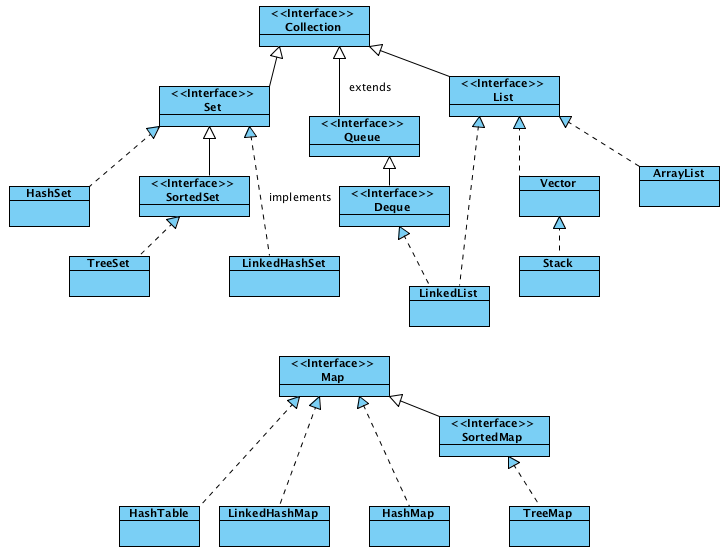
\includegraphics[width=0.74\linewidth]{img/collections}
\end{figure}

\clearpage

\textbf{Exemplos}

\begin{table}[H]
	\centering
	\begin{tabular}{lll}
		\hline
		\textbf{Estrutura} & \textbf{Interface} & \textbf{Implementações} \\
		\hline
		Pilha & \texttt{List} & \texttt{Stack} \\
		Fila & \texttt{Queue} & \texttt{LinkedList} \\
		Deque & \texttt{Deque} & \texttt{ArrayDeque}, \texttt{LinkedList} \\
		Lista dinâmica & \texttt{List} & \texttt{ArrayList}, \texttt{LinkedList} \\
		Fila de prioridade & \texttt{Queue} & \texttt{PriorityQueue} \\
		Mapa & \texttt{Map} & \texttt{HashTable}, \texttt{TreeMap} \\
		\hline
	\end{tabular}
\end{table}

\bigskip

\newtitle{Outras estruturas de dados}

\textbf{Tabelas hash}
\begin{itemize}
	\item Outra (e mais eficiente) forma de implementar um mapa.
	\item Também chamado de tabela de dispersão ou tabela de espalhamento.
	\item Utiliza uma \textit{função hash} que mapeia chaves para posições no vetor.
	\item A função calcula a posição que o elemento será/está armazenado.
	\item Operações básicas em tempo constante $O(1)$.
	\item \textbf{Implementação:} \texttt{Map}, \texttt{Hashtable}, \texttt{LinkedHashMap}, \texttt{HashMap}.
	\item \textbf{Operações:} \texttt{put}, \texttt{get}, \texttt{containsKey}, \texttt{remove}.
\end{itemize}

\clearpage

\textbf{Conjuntos}
\begin{itemize}
	\item Estrutura que armazena elementos sem repetição.
	\item Permite operações realizadas sobre conjuntos.
	\item \textbf{Implementação:} \texttt{Set}, \texttt{SortedSet}, \texttt{HashSet}.
	\item \textbf{Operações:} \texttt{add}, \texttt{contains}, \texttt{remove}, \texttt{addAll}, \texttt{removeAll}, \texttt{retainAll}.
\end{itemize}

\bigskip

\textbf{Multiconjuntos}
\begin{itemize}
	\item Trata-se de um conjunto que permite repetição de elementos.
	\item Também conhecido como \textit{bag}.
	\item A ordem é irrelevante: \texttt{\{a, b, c\} = \{b, c, a\}}.
	\item \textbf{Implementação:} utiliza-se um \texttt{ArrayList<E>} ou um \texttt{Map<E, Integer>} (contando os elementos).
	\item \textbf{Operações:} iguais às dos conjuntos.
\end{itemize}

\bigskip

\textbf{Multimapas}
\begin{itemize}
	\item Trata-se de um mapa que armazena múltiplos valores para uma mesma chave.
	\item \textbf{Implementação:} um mapa que permite repetição de chave, ou um mapa cuja entrada armazena a chave e uma lista de valores.
	\item \textbf{Operações:} iguais às dos mapas.
\end{itemize}

\clearpage

\newtitle{Classe Arrays}

\begin{itemize}
	\item A classe \texttt{java.util.Arrays} fornece implementação de vários métodos úteis no tratamento de coleções.
\end{itemize}

\begin{table}[H]
	\centering
	\begin{tabular}{ll}
		\hline
		\textbf{Método} & \textbf{Descrição} \\
		\hline
		\texttt{asList} & dado um vetor, devolve uma lista encadeada. \\
		\texttt{binarySearch} & executa uma busca binária na coleção recebida. \\
		\texttt{copyOf} & retorna uma cópia da coleção recebida. \\
		\texttt{equals} & compara se duas estruturas são iguais. \\
		\texttt{fill} & preenche a coleção pelo valor recebido. \\
		\texttt{sort} & ordena a coleção recebida. \\
		\texttt{toString} & devolve uma String com os elementos da coleção. \\
		\hline
	\end{tabular}
\end{table}

\medskip

\newtitle{Atividades}

\begin{enumerate}
	\item Refaça os exercícios de implementação utilizando as estruturas fornecidas pelo framework \texttt{java.util.Collections}.
	
	\item Desenvolva um programa para armazenar dados utilizando tabelas hash, conjuntos, multiconjuntos e multimapas. Explore as operações fornecidas pelo framework para essas estruturas de dados.
	
	\item Desenvolva um software que armazene produtos em um \texttt{ArrayList}. Utilize os métodos utilitários da classe \texttt{java.util.Arrays} para manipulação dessa estrutura.
\end{enumerate}

\clearpage

\newtitle{Referências}
\begingroup
	\footnotesize
	\renewcommand{\chapter}[2]{}%
	\bibliographystyle{apalike}
	\bibliography{../referencias}
\endgroup

\end{document}